\chapter{Especificación léxica}

\section{Introducción}
En este capítulo utilizaremos la gramática desarrollada en el capítulo anterior y realizaremos el diseño de un analizador léxico. El objetivo es recorrer la cadena de entrada carácter por carácter y detectar los {\bf tokens} especificados, en este caso Pascal reducido (definido por la gramática).
Para ello, se indicarán como están formados los \emph{tokens}, que son elementos que utilizará el analizador sintáctico posteriormente, y se mostrará el diseño de un autómata que permita el reconocimiento de tales tokens en un recorrido [\ref{sec:lexico_reconocedor}].

\section{Descripción del problema}
Para esta etapa requerimos especificar en un principio el alfabeto que tendrá nuestra cadena de entrada, luego debemos definir que combinación de símbolos corresponderán a lexemas de nuestro lenguaje y partir de estos debemos generar patrones que identifiquen para cada token que lexemas les corresponden [\ref{sec:lexico_definicion}].

Dados los tokens y sus patrones representativos, se especifica un autómata finito determinístico que lee cada símbolo de la cadena de entrada y permite determinar si es un token válido del lenguaje. Para ello el autómata se realiza mediante la unión de autómatas más simples para reconocer los patrones de cada token por separado.

\section{Definición del alfabeto, lexemas, tokens y patrones}
\label{sec:lexico_definicion}
El alfabeto estará compuesto por las letras del abecedario (A-Z y a-z) en conjunción con los dígitos de 0-9 y algunos caracteres especiales:

$$ \Sigma = \{ \bm{A}, ..., \bm{Z}, \bm{a}, ..., \bm{z}, \bm{0}, ..., \bm{9}, \bm{\_}, \bm{\}}, \bm{\{}, \bm{)}, \bm{(}, \bm{;}, \bm{\cdot}, \bm{,}, \bm{:}, \bm{=}, \bm{<}, \bm{>}, \bm{+}, \bm{-}, \bm{*}, \bm{/} \}$$

Con estos símbolos podemos definir los lexemas que componen el subconjunto de lenguaje Pascal que se desarrolla y luego definir expresiones regulares para poder identificar a que token corresponden.

En la tabla \ref{tab:tabla_token} podemos visualizar los token que se indentifican en el lenguaje especificado junto con los patrones que definen los lexemas que se corresponden con cada uno de estos token. Tales patrones se especificarán mediante expresiones regulares.

\begin{table}[H]
\centering
\begin{tabular}{|l|l|l|}
\rowcolor{gray!20}
\hline
Token         & Patrón                                               & Ejemplo              \\ \hline
tk\_type\_int      & $integer$                                  & $integer$            \\ \hline
tk\_type\_bool      & $boolean$                                  & $boolean$            \\ \hline
tk\_boolean\_true   & $true$                                       & $true$               \\ \hline
tk\_boolean\_false   & $false$                                       & $false$               \\ \hline
tk\_number   & $[0-9]^+$                                            & $100$                \\ \hline
tk\_id        & $([A-Z] | [a-z] | \_)([A-Z] | [a-z] | \_ | [0-9])^*$ & $un\_identificador\_1$ \\ \hline
tk\_assign    & $:=$                                                 & $:=$                 \\ \hline
tk\_rel\_op\_eq   & $=$                           & $=$                 \\ \hline
tk\_rel\_op\_neq   & $<>$                           & $<>$                 \\ \hline
tk\_rel\_op\_min   & $<$                           & $<$                 \\ \hline
tk\_rel\_op\_may   & $>$                           & $>$                 \\ \hline
tk\_rel\_op\_leq   & $<=$                           & $<=$                 \\ \hline
tk\_rel\_op\_geq   & $>=$                           & $>=$                 \\ \hline
tk\_add\_op\_sum   & $+$                                             & $+$                  \\ \hline
tk\_add\_op\_rest   & $-$                                             & $-$                  \\ \hline
tk\_mult\_op\_por  & $*$                                              & $*$                  \\ \hline
tk\_mult\_op\_div  & $/$                                              & $/$                  \\ \hline
tk\_bool\_op\_and  & $and$                                           & $and$                \\ \hline
tk\_bool\_op\_or  & $or$                                           & $or$                \\ \hline
tk\_not\_op   & $not$                                                & $not$                \\ \hline
tk\_if        & $if$                                                 & $if$                 \\ \hline
tk\_then      & $then$                                               & $then$               \\ \hline
tk\_else      & $else$                                               & $else$               \\ \hline
tk\_while     & $while$                                              & $while$              \\ \hline
tk\_do        & $do$                                                 & $do$                 \\ \hline
tk\_program   & $program$                                            & $program$            \\ \hline
tk\_begin     & $begin$                                              & $begin$              \\ \hline
tk\_end       & $end$                                                & $end$                \\ \hline
tk\_var       & $var$                                                & $var$                \\ \hline
tk\_procedure & $procedure$                                          & $procedure$          \\ \hline
tk\_function  & $function$                                           & $function$           \\ \hline
tk\_read  & $read$                                           & $read$           \\ \hline
tk\_write  & $write$                                           & $write$           \\ \hline
tk\_opar      & (                                                    & (                    \\ \hline
tk\_cpar      & )                                                    & )                    \\ \hline
tk\_tpoints   & :                                                    & :                    \\ \hline
tk\_endstnc   & ;                                                    & ;                    \\ \hline
tk\_point     & .                                                    & .                    \\ \hline
tk\_comma     & ,                                                    & ,                    \\ \hline
\end{tabular}
\caption{Define para cada token el patrón que identifica los lexemas que le corresponden.}
\label{tab:tabla_token}
\end{table}

\section{Estrategias}
Utilizamos diferentes tokens para cada uno de los operadores, como en los operadores de comparación, de multiplicación, y de suma. Así aunque se manejen mas cantidad de tokens que si estuvieren agrupados, es mas sencillo diferenciarlos en las etapas posteriores.

Para componer el reconocedor, tomaremos cualquier cadena de entrada que pueda ser una palabra clave, con el patrón del token id. Si es una palabra clave, se crea su token correspondiente, si no lo es, entonces se confirma que es un id. De esta manera se simplifica el autómata reconocedor de tokens.

\section{Limitaciones}
\label{sec:lexico_limitaciones}
En la especificación de tokens se ha indicado para cada operador un token diferente, como con los operadores relacionales (rel\_op), esto permite diferenciarlos y en futuras etapas facilita la implementación. En cambio se pudo optar por una visión mas genérica que facilite la visualización de los diferentes token conceptualmente, de manera que queden agrupados y se diferencien por un atributo que indique específicamente que lexema representa.

Por otro lado, con respecto al diseño del autómata, se consideró, para simplificar el diseño, que las palabras reservadas no serán reconocidas por estados independientes si no que serán un caso específico del patrón para reconocer identificadores (tk\_id).

\section{Diseño del reconocedor}
\label{sec:lexico_reconocedor}

% \begin{figure}[H]
% \begin{center}
% \begin{tikzpicture}[scale=0.15]
% \tikzstyle{every node}+=[inner sep=0pt]
% \draw [black] (49,-15.4) circle (3);
% \draw (49,-15.4) node {$2$};
% \draw [black] (49,-2.8) circle (3);
% \draw (49,-2.8) node {$1$};
% \draw [black] (64.8,-15.4) circle (3);
% \draw (64.8,-15.4) node {$3\mbox{ }*$};
% \draw (76,-15.4) node {{\bf return($tk\_id$)}};
% \draw [black] (64.8,-15.4) circle (2.4);
% \draw [black] (22.5,-2.8) circle (3);
% \draw (22.5,-2.8) node {$start$};
% \draw [black] (49,-28.4) circle (3);
% \draw (49,-28.4) node {$4$};
% \draw [black] (65.4,-28.4) circle (3);
% \draw (65.4,-28.4) node {$5\mbox{ }*$};
% \draw (78.5,-28.4) node {{\bf return($tk\_integer$)}};
% \draw [black] (65.4,-28.4) circle (2.4);
% \draw [black] (49,-38.3) circle (3);
% \draw (49,-38.3) node {$6$};
% \draw [black] (65.4,-42.6) circle (3);
% \draw (65.4,-42.6) node {$7$};
% \draw (78.5,-42.6) node {{\bf return($tk\_assign$)}};
% \draw [black] (65.4,-42.6) circle (2.4);
% \draw [black] (48.5,-47.4) circle (3);
% \draw (48.5,-47.4) node {$8$};
% \draw (63.4,-46.9) node {{\bf return($tk\_rel\_op\_eq$)}};
% \draw [black] (48.5,-47.4) circle (2.4);
% \draw [black] (48.5,-56.2) circle (3);
% \draw (48.5,-56.2) node {$9$};
% \draw [black] (65.4,-51.7) circle (3);
% \draw (65.4,-51.7) node {$10\mbox{ }*$};
% \draw (80,-51.7) node {{\bf return($tk\_rel\_op\_min$)}};
% \draw [black] (65.4,-51.7) circle (2.4);
% \draw [black] (65.4,-59.1) circle (3);
% \draw (65.4,-59.1) node {$11$};
% \draw (80,-59.1) node {{\bf return($tk\_rel\_op\_leq$)}};
% \draw [black] (65.4,-59.1) circle (2.4);
% \draw [black] (65.4,-66) circle (3);
% \draw (65.4,-66) node {$12$};
% \draw (80,-66) node {{\bf return($tk\_rel\_op\_neq$)}};
% \draw [black] (65.4,-66) circle (2.4);
% \draw [black] (48.5,-72.8) circle (3);
% \draw (48.5,-72.8) node {$13$};
% \draw [black] (65.4,-72.8) circle (3);
% \draw (65.4,-72.8) node {$14$};
% \draw (80,-72.8) node {{\bf return($tk\_rel\_op\_geq$)}};
% \draw [black] (65.4,-72.8) circle (2.4);
% \draw [black] (65.4,-80.7) circle (3);
% \draw (65.4,-80.7) node {$15\mbox{ }*$};
% \draw (80,-80.7) node {{\bf return($tk\_rel\_op\_may$)}};
% \draw [black] (65.4,-80.7) circle (2.4);
% \draw [black] (49,-86.4) circle (3);
% \draw (49,-86.4) node {$16$};
% \draw (63,-86.4) node {{\bf return($tk\_add\_op$)}};
% \draw [black] (49,-86.4) circle (2.4);
% \draw [black] (49,-95.6) circle (3);
% \draw (49,-95.6) node {$18$};
% \draw (63,-95.6) node {{\bf return($tk\_mult\_op$)}};
% \draw [black] (49,-95.6) circle (2.4);
% \draw [black] (65.4,-35.7) circle (3);
% \draw (65.4,-35.7) node {$19\mbox{ }*$};
% \draw (78.5,-35.7) node {{\bf return($tk\_tpoins$)}};
% \draw [black] (65.4,-35.7) circle (2.4);
% \draw [black] (51.253,-0.837) arc (158.78564:-129.21436:2.25);
% \draw (56.29,-0.58) node [right] {$otro$};
% \fill [black] (51.93,-3.39) -- (52.49,-4.15) -- (52.86,-3.22);
% \draw [black] (47.677,-12.72) arc (234:-54:2.25);
% \draw (49,-8.15) node [above] {$letter\mbox{ }or\mbox{ }digit\mbox{ }or\mbox{ }\_$};
% \fill [black] (50.32,-12.72) -- (51.2,-12.37) -- (50.39,-11.78);
% \draw [black] (52,-15.4) -- (61.8,-15.4);
% \fill [black] (61.8,-15.4) -- (61,-14.9) -- (61,-15.9);
% \draw (56.9,-14.9) node [above] {$otro$};
% \draw [black] (46,-2.8) -- (25.5,-2.8);
% \fill [black] (25.5,-2.8) -- (26.3,-3.3) -- (26.3,-2.3);
% \draw (35.75,-3.3) node [below] {$\}$};
% \draw [black] (25.231,-1.562) arc (111.4063:68.5937:28.821);
% \fill [black] (46.27,-1.56) -- (45.71,-0.8) -- (45.34,-1.74);
% \draw (35.75,0.93) node [above] {$\{$};
% \draw [black] (25.21,-4.09) -- (46.29,-14.11);
% \fill [black] (46.29,-14.11) -- (45.78,-13.32) -- (45.35,-14.22);
% \draw (31.15,-9.63) node [below] {$letter\mbox{ }or\mbox{ }\_$};
% \draw [black] (46.059,-27.813) arc (-103.99149:-164.0292:31.782);
% \fill [black] (46.06,-27.81) -- (45.4,-27.13) -- (45.16,-28.1);
% \draw (29.31,-20.31) node [below] {$digit$};
% \draw [black] (47.677,-25.72) arc (234:-54:2.25);
% \draw (49,-21.15) node [above] {$digit$};
% \fill [black] (50.32,-25.72) -- (51.2,-25.37) -- (50.39,-24.78);
% \draw [black] (52,-28.4) -- (62.4,-28.4);
% \fill [black] (62.4,-28.4) -- (61.6,-27.9) -- (61.6,-28.9);
% \draw (57.2,-28.9) node [below] {$otro$};
% \draw [black] (46.002,-38.324) arc (-92.79513:-193.72375:26.42);
% \fill [black] (46,-38.32) -- (45.23,-37.79) -- (45.18,-38.78);
% \draw (25.54,-29.13) node [left] {$:$};
% \draw [black] (51.9,-39.06) -- (62.5,-41.84);
% \fill [black] (62.5,-41.84) -- (61.85,-41.15) -- (61.6,-42.12);
% \draw (58,-39.88) node [above] {$=$};
% \draw [black] (45.501,-48.422) arc (-92.52263:-208.09592:29.287);
% \fill [black] (45.5,-48.42) -- (44.72,-47.89) -- (44.68,-48.89);
% \draw (20.69,-34.89) node [left] {$=$};
% \draw [black] (45.517,-56.504) arc (-86.95094:-221.12695:31.119);
% \fill [black] (45.52,-56.5) -- (44.69,-56.05) -- (44.74,-57.05);
% \draw (15.18,-40.13) node [left] {$<$};
% \draw [black] (51.4,-55.43) -- (62.5,-52.47);
% \fill [black] (62.5,-52.47) -- (61.6,-52.19) -- (61.86,-53.16);
% \draw (55.34,-53.32) node [above] {$otro$};
% \draw [black] (51.46,-56.71) -- (62.44,-58.59);
% \fill [black] (62.44,-58.59) -- (61.74,-57.96) -- (61.57,-58.95);
% \draw (56.46,-58.25) node [below] {$=$};
% \draw [black] (51.1,-57.7) -- (62.8,-64.5);
% \fill [black] (62.8,-64.5) -- (62.36,-63.66) -- (61.86,-64.53);
% \draw (55.89,-61.6) node [below] {$>$};
% \draw [black] (45.516,-72.502) arc (-97.80406:-221.44306:40.861);
% \fill [black] (45.52,-72.5) -- (44.79,-71.9) -- (44.66,-72.89);
% \draw (12,-47.06) node [left] {$>$};
% \draw [black] (51.5,-72.8) -- (62.4,-72.8);
% \fill [black] (62.4,-72.8) -- (61.6,-72.3) -- (61.6,-73.3);
% \draw (56.95,-73.3) node [below] {$=$};
% \draw [black] (51.22,-74.07) -- (62.68,-79.43);
% \fill [black] (62.68,-79.43) -- (62.17,-78.64) -- (61.75,-79.54);
% \draw (54.87,-77.27) node [below] {$otro$};
% \draw [black] (46.068,-85.769) arc (-103.8764:-220.94786:49.664);
% \fill [black] (46.07,-85.77) -- (45.41,-85.09) -- (45.17,-86.06);
% \draw (9.87,-53.22) node [left] {$+\mbox{ }or\mbox{ }-$};
% \draw [black] (46.027,-95.204) arc (-99.23615:-228.88937:51.996);
% \fill [black] (46.03,-95.2) -- (45.32,-94.58) -- (45.16,-95.57);
% \draw (3.61,-58.72) node [left] {$*\mbox{ }or\mbox{ }/$};
% \draw [black] (19.572,-3.399) arc (309.29645:21.29645:2.25);
% \draw (15.21,-0.59) node [left] {$ws$};
% \fill [black] (20.24,-0.84) -- (20.12,0.1) -- (19.35,-0.54);
% \draw [black] (51.96,-37.83) -- (62.44,-36.17);
% \fill [black] (62.44,-36.17) -- (61.57,-35.8) -- (61.73,-36.79);
% \draw (56.34,-36.3) node [above] {$otro$};
% \end{tikzpicture}
% \end{center}
% \caption{Autómata reconocedor de tokens.}
% \label{fig:automata_token2}
% \end{figure}

\begin{figure}[H]
\centering
\begin{tikzpicture}[scale=0.65, node distance = 2.5cm, state/.style={circle, draw, minimum size=1cm}]
\tikzset{every state/.append style={thick, fill=gray!10}}
\node[state] (0) at (0,0) {$start$};
\node[state] (1) at (0,-6) {$1$};
\node[state] (2) at (3,6) {$2$};
\node[state, accepting] (3) at (6,6) {$3$ $*$};
\node[state] (4) at (3,2) {$4$};
\node[state, accepting] (5) at (6,4) {$5$ $*$};
\node[state] (6) at (3,0) {$6$};
\node[state, accepting] (7) at (6,2) {$7$ $*$};
\node[state, accepting] (8) at (6,0) {$8$};
\node[state] (9) at (3,-4) {$9$};
\node[state, accepting] (10) at (6,-2) {$10$ $*$};
\node[state, accepting] (11) at (6,-4) {$11$};
\node[state, accepting] (12) at (6,-6) {$12$};
\node[state] (13) at (-3,5) {$13$};
\node[state, accepting] (14) at (-6,6) {$14$ $*$};
\node[state, accepting] (15) at (-6,4) {$15$};
\node[state, accepting] (16) at (-6,2) {$16$};
\node[state, accepting] (17) at (-6,0) {$17$};
\node[state, accepting] (18) at (-6,-2) {$18$};
\node[state, accepting] (19) at (-6,-4) {$19$};
\node[state, accepting] (20) at (-6,-6) {$20$};

\node[right] at (7,6) {{\bf return($tk\_id$)}};
\node[right] at (7,4) {{\bf return($tk\_number$)}};
\node[right] at (7,2) {{\bf return($tk\_tpoints$)}};
\node[right] at (7,0) {{\bf return($tk\_assign$)}};
\node[right] at (7,-2) {{\bf return($tk\_rel\_op\_min$)}};
\node[right] at (7,-4) {{\bf return($tk\_rel\_op\_leq$)}};
\node[right] at (7,-6) {{\bf return($tk\_rel\_op\_neq$)}};

\node[left] at (-7,6) {{\bf return($tk\_rel\_op\_may$)}};
\node[left] at (-7,4) {{\bf return($tk\_rel\_op\_geq$)}};
\node[left] at (-7,2) {{\bf return($tk\_rel\_op\_eq$)}};
\node[left] at (-7,0) {{\bf return($tk\_add\_op\_sum$)}};
\node[left] at (-7,-2) {{\bf return($tk\_add\_op\_rest$)}};
\node[left] at (-7,-4) {{\bf return($tk\_mult\_op\_por$)}};
\node[left] at (-7,-6) {{\bf return($tk\_mult\_op\_div$)}};

\path[->,>=stealth]
(0) edge[loop above] node{$ws$} (0)	
	edge[bend left, left] node{$\{$} (1)
    edge[above] node{$letter$ or $\_$} (2)
    edge[above] node{$digit$} (4)
    edge[above] node{$:$} (6)
    edge[above] node{$<$} (9)
    edge[left] node{$>$} (13)
    edge[above] node{$=$} (16)
    edge[above] node{$+$} (17)
    edge[above] node{$-$} (18)
    edge[above] node{$*$} (19)
    edge[above] node{$/$} (20)
(1) edge[loop below] node{$otro$} (1)
	edge[bend left, right] node{$\}$} (0)
(2) edge[loop above] node{$letter$ or $digit$ or $\_$} (2)
	edge[above] node{$otro$} (3)
(4) edge[loop above] node{$digit$} (4)
	edge[above] node{$otro$} (5)
(6) edge[above] node{$otro$} (7)
	edge[above] node{$=$} (8)
(9) edge[above] node{$otro$} (10)
	edge[above] node{$=$} (11)
	edge[above] node{$>$} (12)
(13) edge[above] node{$otro$} (14)
	 edge[above] node{$=$} (15)
;
\end{tikzpicture}
\caption{Autómata reconocedor de tokens.}
\label{fig:automata_token}
\end{figure}

Podemos contemplar que en ciertos estados se consume un elemento \emph{otro}, el cuál dependerá de tal estado, y simboliza un elemento que no corresponde con los símbolos cuyos lexemas están incluidos en el patrón del token que está reconociendo. Por ejemplo, en el arco del estado 2-3, \emph{otro} corresponde a símbolos que no son \emph{letter}, \emph{digit} o \emph{\_}. En el caso del arco 4-5 corresponde un símbolo que no es \emph{digit}. En 9-10 para cualquier símbolo que no es \emph{=} o \emph{$>$} y en 13-15 para cualquiera que no sea \emph{=}. Finalmente en el arco del estado 1, se utiliza de manera que reconozca cualquier símbolo, ya que este es el encargado de reconocer las secciones comentadas del código, lo que permite ignorar cualquier símbolo encerrado entre llaves.

Por otro lado, encontramos el arco etiquetado con \emph{ws} que permite ignorar los espacios, los saltos de línea y las tabulaciones.

A modo de simplificación del gráfico, tanto por cuestiones de tamaño como de estética, no se indicó el reconocimiento de los siguientes tokens: tk\_opar, tk\_cpar, tk\_tpoints, tk\_endstnc, tk\_point, tk\_comma. Estos patrones son triviales, y serían análogos, por ejemplo, al reconocimiento de tk\_mult\_op.
%\section{Problemas encontrados}

\section{Implementación del aplicativo}
\label{sec:implementacion_lexico}
En esta sección proponemos una implementación de un analizador léxico que se corresponde con la especificación léxica de la sección anterior.

Se dispondrá el enlace del código fuente alojado en GitHub\footnote{\url{https://github.com/Martinnqn/CompiladorPascal}}. Durante el desarrollo de este trabajo se ampliará el aplicativo con las demás etapas de análisis sintáctico y semántico. De esta manera, esperamos concluir todas las etapas del compilador para el lenguaje elegido.  

\subsection{Descripción del problema}
La idea es desarrollar y documentar un programa capaz de reconocer lexemas de un código fuente basado en la gramática de la sección \ref{sec:definicion_gramatica}, y devolver sus tokens asociados en la tabla \ref{tab:tabla_token}. Para esto, usaremos el autómata de la figura \ref{fig:automata_token}.

\subsection{Herramientas utilizadas} %ver titulo..
Para desarrollar el programa escogimos el lenguaje Java. La versión de Java sobre la que trabajamos es la 8\footnote{Actualización 171, al día 14/05/2018}(ocho), sobre el sistema operativo Windows 10. 

El código de fuente alojado en GitHub tiene la estructura de un proyecto de NetBeans, por lo que puede usarse ese IDE para levantar el proyecto.

\subsection{Diseño}
Para llevar a cabo lo propuesto en este capítulo, y luego poder continuar con el mismo proyecto ampliando el código con las siguientes etapas de análisis, propusimos estructurar el proyecto en \emph{packages}. La estructura del proyecto se puede ver en la figura \ref{fig:arbol_dir}, por lo que ahora nos centraremos en trabajar sobre el paquete \emph{lexico}, el cual contiene todas las clases que se usarán en el análisis léxico.

\begin{figure}[H]
%no borrar el % de dirtree porque es necesario.
\dirtree{%
.1 src.
.2 compiladorpascal.
.3 CompiladorPascal.java.
.3 lexico.
.3 sintactico.
.3 semantico.
}
\caption{Árbol de directorios del proyecto de Java.}
\label{fig:arbol_dir}
\end{figure}
La clase {\bf CompiladorPascal} será la clase principal del proyecto, donde se crearan los objetos necesarios en cada etapa del análisis. 

Las clases que se usarán en el análisis léxico son: {\bf AnalizadorLexico, Token, Tokens}. El árbol de directorios actualizado queda como el de la figura \ref{fig:arbol_dir_2}:
\begin{figure}[H]
%no borrar el % de dirtree porque es necesario.
\dirtree{%
.1 src.
.2 compiladorpascal.
.3 CompiladorPascal.java.
.3 lexico.
.4 AnalizadorLexico.java.
.4 Token.java.
.4 Tokens.java.
.3 sintactico.
.3 semantico.
}
\caption{Árbol de directorios del proyecto de Java con los archivos del analizador léxico.}
\label{fig:arbol_dir_2}
\end{figure}

{\bf Descripción de las clases}: 
\begin{itemize}
\item {\bf AnalizadorLexico}: contiene el código necesario para reconocer cada token y reportar los errores léxicos en caso de haberlos. El código tiene una relación directa con el autómata de la figura \ref{fig:automata_token}.
%\item {\bf ErrorLéxico}: contiene atributos necesarios para mostrar mensajes detallados acerca de los errores léxicos que ocurran durante la compilación. Para cada error se sugiere un mensaje apropiado que permita al programador encontrar el error en el código y poder solucionarlo. 
\item {\bf Token}: contiene los atributos que representan un token, tal como su nombre y valor.
\item {\bf Tokens}: contiene métodos estáticos que almacenan en HashMaps los nombres y valores de los tokens como palabras reservadas y símbolos. Se utilizará en el AnalizadorLexico para obtener los nombres y patrones de los token del lenguaje.
\end{itemize}

%\subsubsection{Estrategias}

%\subsubsection{Limitaciones}

%\subsubsection{Problemas encontrados}

\subsection{Instructivos de instalación y uso}
Al ser un programa hecho en Java, cuenta con la capacidad de ser portable, por lo que no requiere instalación.

El proceso de compilación puede realizarse mediante un IDE (NetBeans en nuestro caso), o mediante la consola o terminal, con el comando \emph{javac *.java} sobre los archivos del paquete.   

\subsection{Ejemplos}
En la figura \ref{fig:lexico_ej_correcto} vemos un programa en nuestro Pascal que es léxicamente correcto, por lo que la salida en la figura \ref{fig:lexico_ej_correcto_salida} nos muestra una cadena con los tokens obtenidos tras el análisis y no menciona ningún error encontrado. Por otro lado en las figura \ref{fig:lexico_ej_error_1} encontramos un código con un caracter desconocido ``$\%$'' y en la figura \ref{fig:lexico_ej_error_1_salida} la correspondiente salida con el error, indicando la línea y posición donde ocurrió y más abajo los tokens que reconoció hasta alcanzar el error. También podemos ver en la figura \ref{fig:lexico_ej_error_2} un código donde no se cierra el comentario por lo que en la figura \ref{fig:lexico_ej_error_2_salida} vemos que la salida es un error específico para este caso.

\begin{figure}[H]
\begin{minted}[autogobble,linenos,xleftmargin=0.35\textwidth,xrightmargin=0.35\textwidth]{pascal}
Program Example1;
Var       
    Num1, Num2, Sum : Integer;
    Result: Boolean;
Begin {no semicolon}
    Sum := Num1 + Num2;
    if (Num1 > Num2) then
        Result := true
End.
\end{minted}
\caption{Programa en Pascal reducido léxicamente correcto.}
\label{fig:lexico_ej_correcto}
\end{figure}

\begin{figure}[H]
\centering
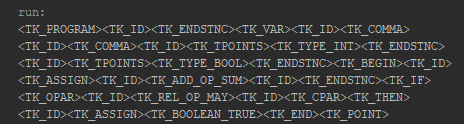
\includegraphics[scale=1]{img/lexico/salida_lexico_ej_correcto.png}
\caption{Salida de la ejecución del analizador léxico con el código de la figura \ref{fig:lexico_ej_correcto}.}
\label{fig:lexico_ej_correcto_salida}
\end{figure}

\begin{figure}[H]
\begin{minted}[autogobble,linenos,xleftmargin=0.35\textwidth,xrightmargin=0.35\textwidth]{pascal}
Program Example2;
Var       
    %Num1, Num2, Sum : Integer;
    Result: Boolean;
Begin [ {no semicolon}
    Sum := Num1 ++ Num2;
    if (Num1 > Num2) then
        Result := true
]
End.
\end{minted}
\caption{Programa en Pascal con error léxico por caracter desconocido.}
\label{fig:lexico_ej_error_1}
\end{figure}

\begin{figure}[H]
\centering
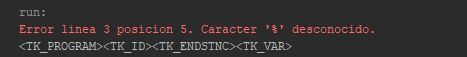
\includegraphics[scale=1]{img/lexico/salida_lexico_ej_error_1.png}
\caption{Salida de la ejecución del analizador léxico con el código de la figura \ref{fig:lexico_ej_error_1}.}
\label{fig:lexico_ej_error_1_salida}
\end{figure}

\begin{figure}[H]
\begin{minted}[autogobble,linenos,xleftmargin=0.35\textwidth,xrightmargin=0.35\textwidth]{pascal}
Program Example3;
Var       
    Num1, Num2, Sum : Integer;
    Result: Boolean;
Begin {no semicolon}
    {Sum := Num1 + Num2;
    if (Num1 > Num2) then
        Result := true
End.
\end{minted}
\caption{Programa en Pascal con error léxico por no encontrar final de comentario.}
\label{fig:lexico_ej_error_2}
\end{figure}

\begin{figure}[H]
\centering
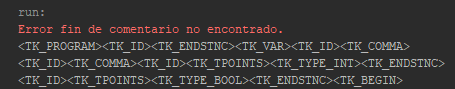
\includegraphics[scale=1]{img/lexico/salida_lexico_ej_error_2.png}
\caption{Salida de la ejecución del analizador léxico con el código de la figura \ref{fig:lexico_ej_error_2}.}
\label{fig:lexico_ej_error_2_salida}
\end{figure}

\section{Conclusiones}
%Realizamos una especificación del autómata de una manera simplificada de manera que sea mas visible su funcionamiento [\ref{sec:lexico_reconocedor}] y a futuro se dará mas detalle a la hora de implementar. De la misma manera para la definición de los token en la tabla \ref{tab:tabla_token} se consideró cada token de una manera mas conceptual y por ello no se especificó uno separado para cada lexema, como se menciona en \ref{sec:lexico_limitaciones}. En este sentido la especificación dada en este capítulo tiene una visión mas general del funcionamiento de un analizador léxico y no tan allegada a la implementación.
En este capítulo pudimos concluir la especificación e implementación del análisis léxico.

Realizamos una definición de los token en la tabla \ref{tab:tabla_token}, considerando cada token conceptualmente como se menciona en \ref{sec:lexico_limitaciones} y así evitamos una definición exhaustiva y simplificamos la tabla.

En base a la tabla de tokens, diseñamos el autómata reconocedor de tokens [\ref{sec:lexico_reconocedor}] describiendo su funcionamiento.

Luego, en la sección \ref{sec:implementacion_lexico}, tuvimos en cuenta las especificaciones y desarrollamos un programa en Java que permite reconocer los tokens de nuestro lenguaje.

En los siguientes capítulos continuaremos desarrollando las especificaciones e implementaciones de las siguientes etapas de un compilador.